\begin{table*}[htbp]
\centering
\caption{Deep Learning Frameworks Used}
\label{table_framework}
\begin{scriptsize}
\begin{tabular}{|l|c|c|l|l|l|}
\hline
  Framework & Version & Multi-GPUs        & \multicolumn{1}{c|}{Operating} & \multicolumn{1}{c|}{User}      & \multicolumn{1}{c|}{Libraries}\\
            &         & (parallelism)     & \multicolumn{1}{c|}{system}    & \multicolumn{1}{c|}{interface} &  \multicolumn{1}{c|}{used} \\
\hline\hline
Caffe      & 1.0.0-rc3 & Data           & Linux          & MATLAB, protobuf, Python & CUDA 7.5, cuDNN 5.0.5 \\\hline
CNTK       & 1.7.2     & Data           & Linux, Windows & BrainScript, C++, C\#    & CUDA 7.5, cuDNN 5.0.5 \\\hline
TensorFlow & 0.10.0rc0 & Data, Model    & Linux          & Python, C++              & CUDA 7.5, cuDNN 5.0.5 \\\hline
Theano     & 0.8.2     & $-$            & Linux          & Python                   & CUDA 7.5, Lasagne 0.2, cuDNN 5.0.5 \\\hline
Torch      & 7         & Data, Model    & Linux          & LuaJIT                   & CUDA 7.5, cuda-convnet3, cuDNN 5.0.5, cuDNN 5.1.3, ccn2.torch \\\hline 
\multicolumn{4}{l}{*All the frameworks spupport a single GPU.}
\end{tabular}
\end{scriptsize}
\end{table*}

\section{Background and Related work}
In this section, we briefly describe the five major deep learning frameworks and a typical organization of CNNs. We also introduce some related studies that perform comparative studies of deep learning frameworks.

\subsection{Deep Learning Frameworks}
There are five major deep learning frameworks that are frequently used by machine learning users to build deep learning models: Caffe\cite{jia2014caffe}, CNTK (Computational Network Toolkit)\cite{cntk}, TensorFlow\cite{tensorflow2015-whitepaper}, Theano\cite{DBLP:journals/corr/Al-RfouAAa16}, and Torch\cite{torch}. Table~\ref{table_framework} summarizes the frameworks used in this paper (we will describe the data parallelism and model parallelism later in this section). 

Visual recognition challenge winners are usually implemented with Caffe\cite{ILSVRC15, RCNN, vgg}. However, the flexibility of Caffe is somehow limited. Introducing a new feature to a layer requires re-building the entire source code. CNTK developed by Microsoft is widening it user base even though it was introduced most recently in 2016. TensorFlow was publicly introduced in 2015 and is now the most popular deep learning framework in GitHub\cite{github}. Theano is one of the earliest deep learning frameworks. Pylearn2\cite{pylearn2}, Keras\cite{keras}, and Lasagne\cite{lasagne} are popular DNN frameworks that use Theano as their backend. However, The Multi-GPU support of Theano is still in an experimental stage. Torch is a scientific computing framework based on LuaJIT\cite{torch} and also one of the earliest DNN frameworks. NVIDIA's self-driving car project\cite{nvdave} and Deepmind's Deep Q Learning model\cite{mnih2015humanlevel} were built on top of it.

\subsection{Convolutions}
A convolution is an operation between two functions. Its value shows the degree of similarity between the two functions $f$ and $g$. Convolutions can also be naturally defined for discrete values. We can define the convolution of two finite sequences $f[n] \; (0 \leq n \leq N-1)$ and $g[j] \; (0 \leq m \leq M-1)$ as follows:
\begin{equation}
\label{def_discrete}
\left ( f * g \right )[n] = \sum_{m=0}^{M-1} f[n + m]g[m]
\end{equation}
The convolution operation can be extended to multiple dimensions. A two-dimensional (2D) convolution between filter (a.k.a. kernel) $F[r][s] \; (0 \leq r \leq R-1, 0 \leq s \leq S-1)$ and data $D[h][w] \; (0 \leq h \leq H-1, 0 \leq w \leq W-1)$ can be described with the following equation:
\begin{equation}
\label{def_2d}
\left ( D * F \right )[h][w] = \sum_{r=0}^{R-1}\sum_{s=0}^{S-1} D[h + r][w + s] F[r][s]
\label{2d-conv}
\end{equation}

\begin{figure}[htbp]
  \centering
  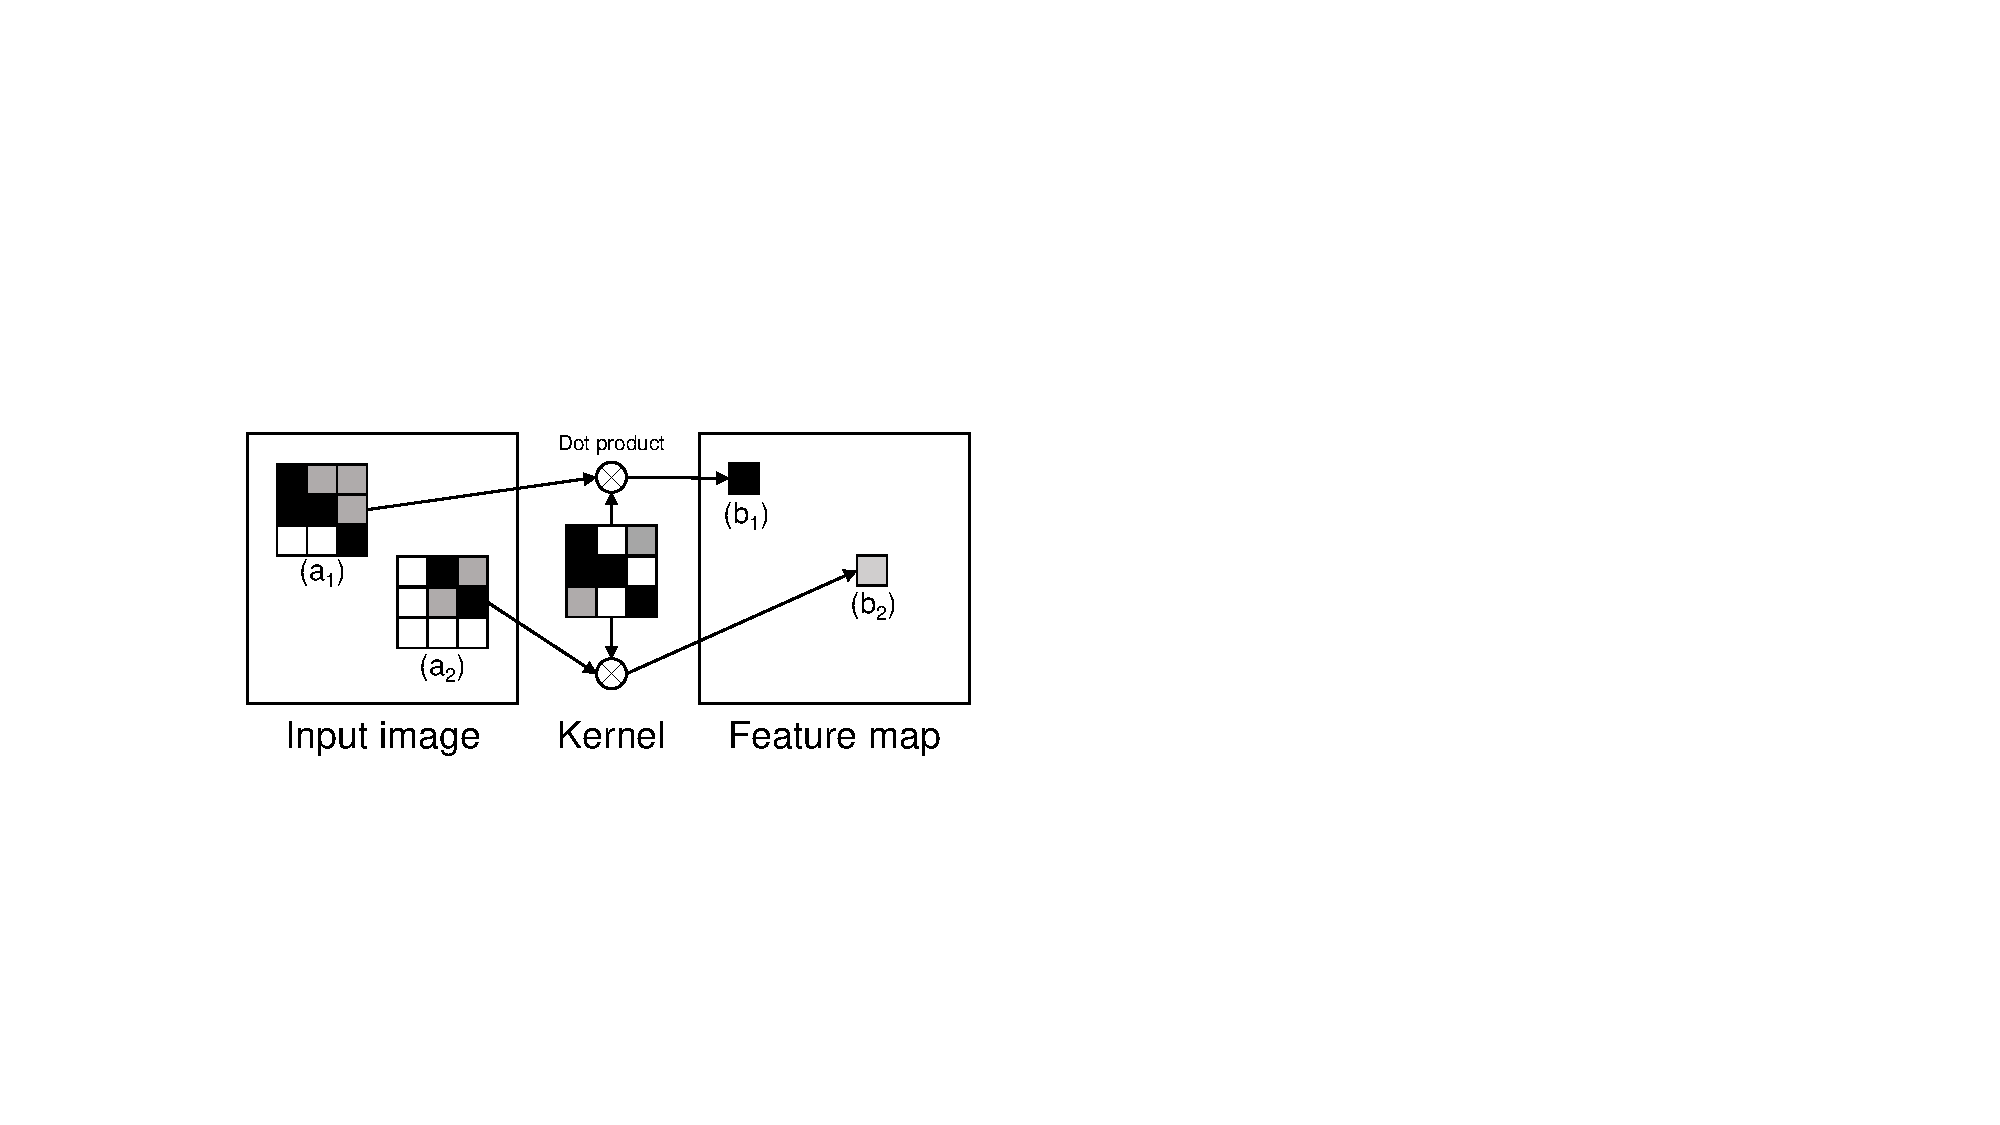
\includegraphics[width=0.6\linewidth]{./figures/feature-map}
  \caption{2D convolution. }
  \label{fig_conv}
\end{figure}

Such a 2D discrete convolution is widely used in image processing and sometimes called an \textit{image convolution}. An image, $D[h][w]$ in Equation~\ref{2d-conv}, is treated as a function of 2D pixel coordinates in an image convolution. $F[h][w]$ in Equation~\ref{2d-conv} is called a filter or a kernel. The result of the 2D convolution generates a feature map as shown in Figure~\ref{fig_conv}. The size of a filter ($R \times S$) is typically much smaller than the input image size ($H \times W$). For a given filter, input image regions (\textit{e.g.}, $a_1$ and $a_2$) with the same size and dimension as the kernel are point-wisely multiplied with the kernel. A \textit{feature map} consists of all the results (\textit{e.g.}, $b_1$ and $b_2$) of such multiplications. A high value of the convolution implies that the corresponding region in the input image has a high degree of similarity to the kernel. 

\begin{figure}[htbp]
  \centering
  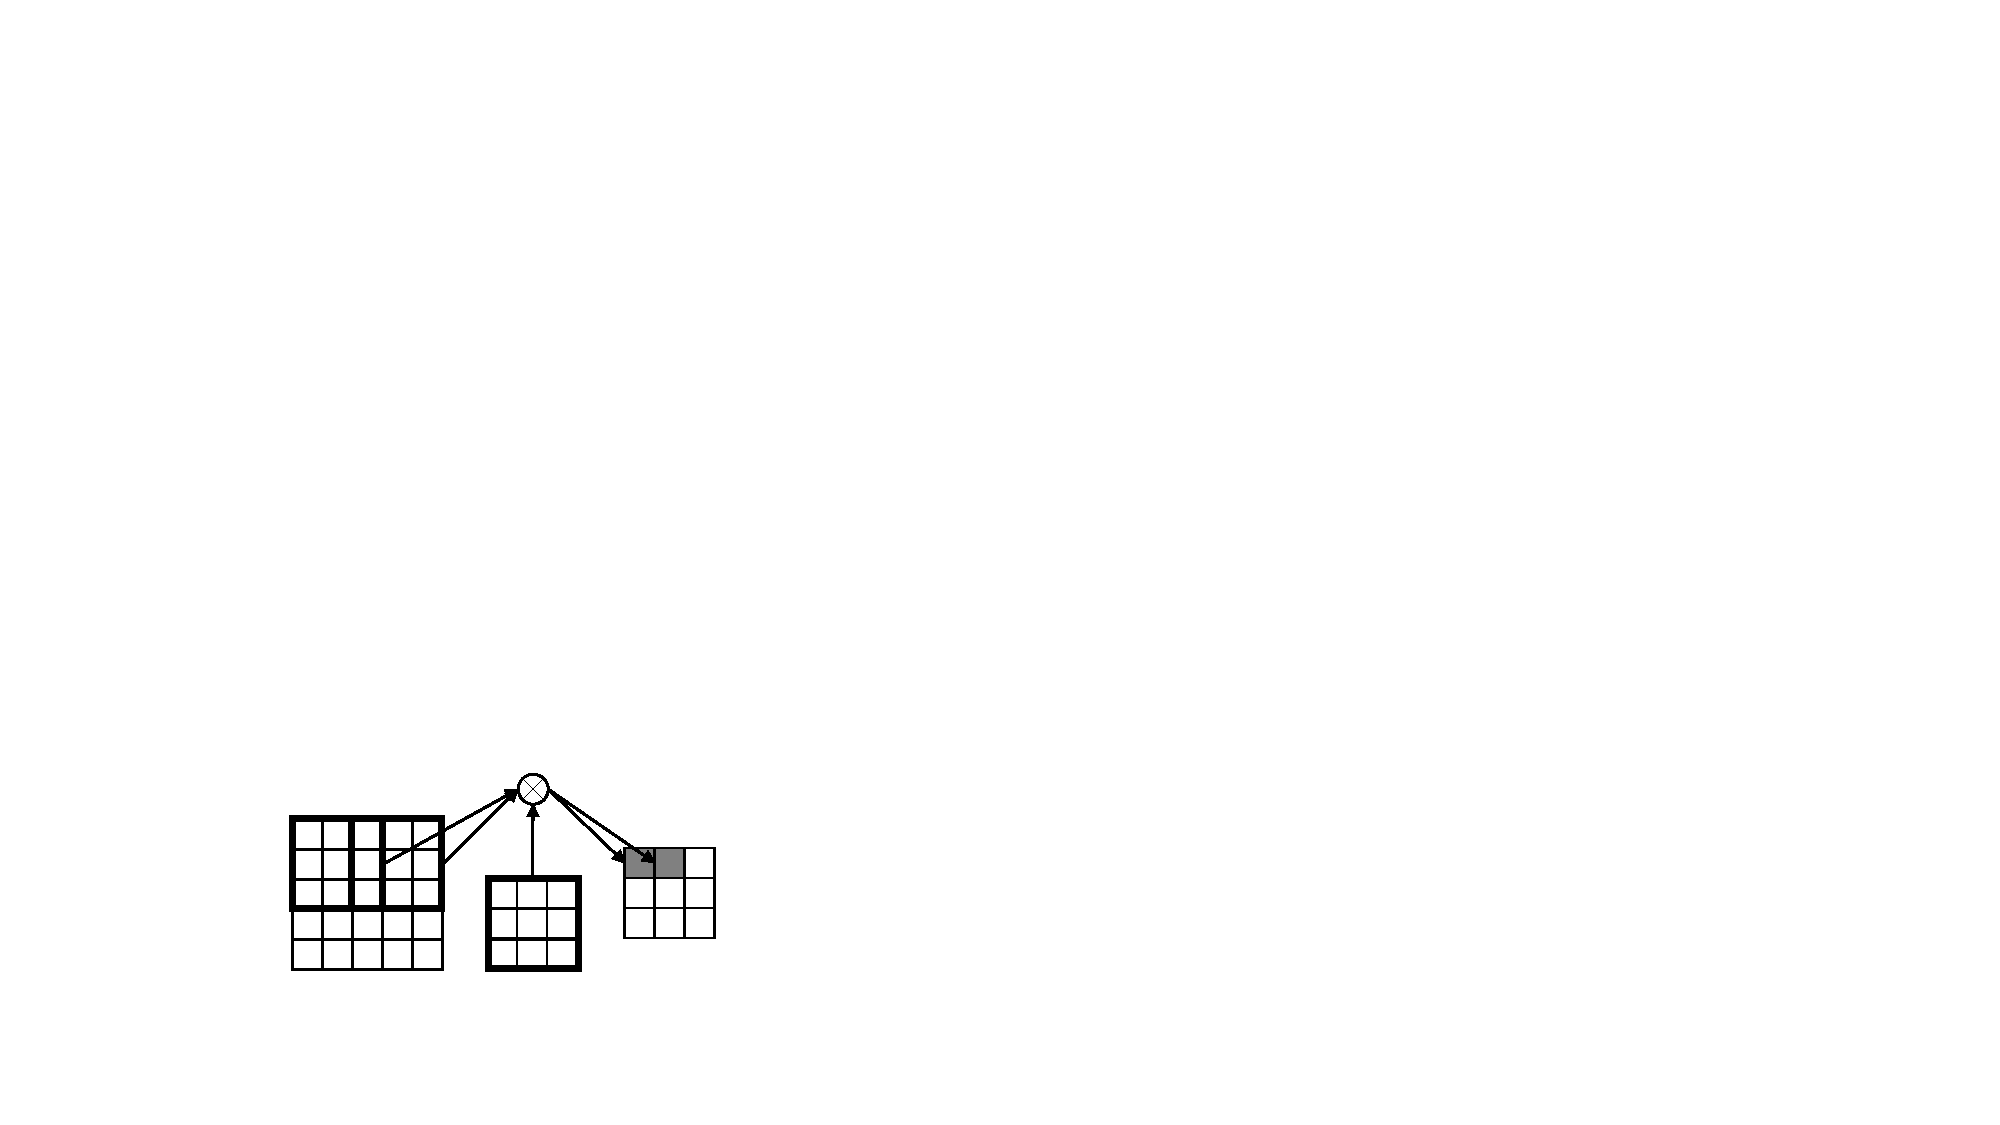
\includegraphics[width=0.5\linewidth]{./figures/stride}
  \caption{Convolution with a stride of two. }
  \label{fig_stride}
\end{figure}

\begin{figure}[htbp]
  \centering
  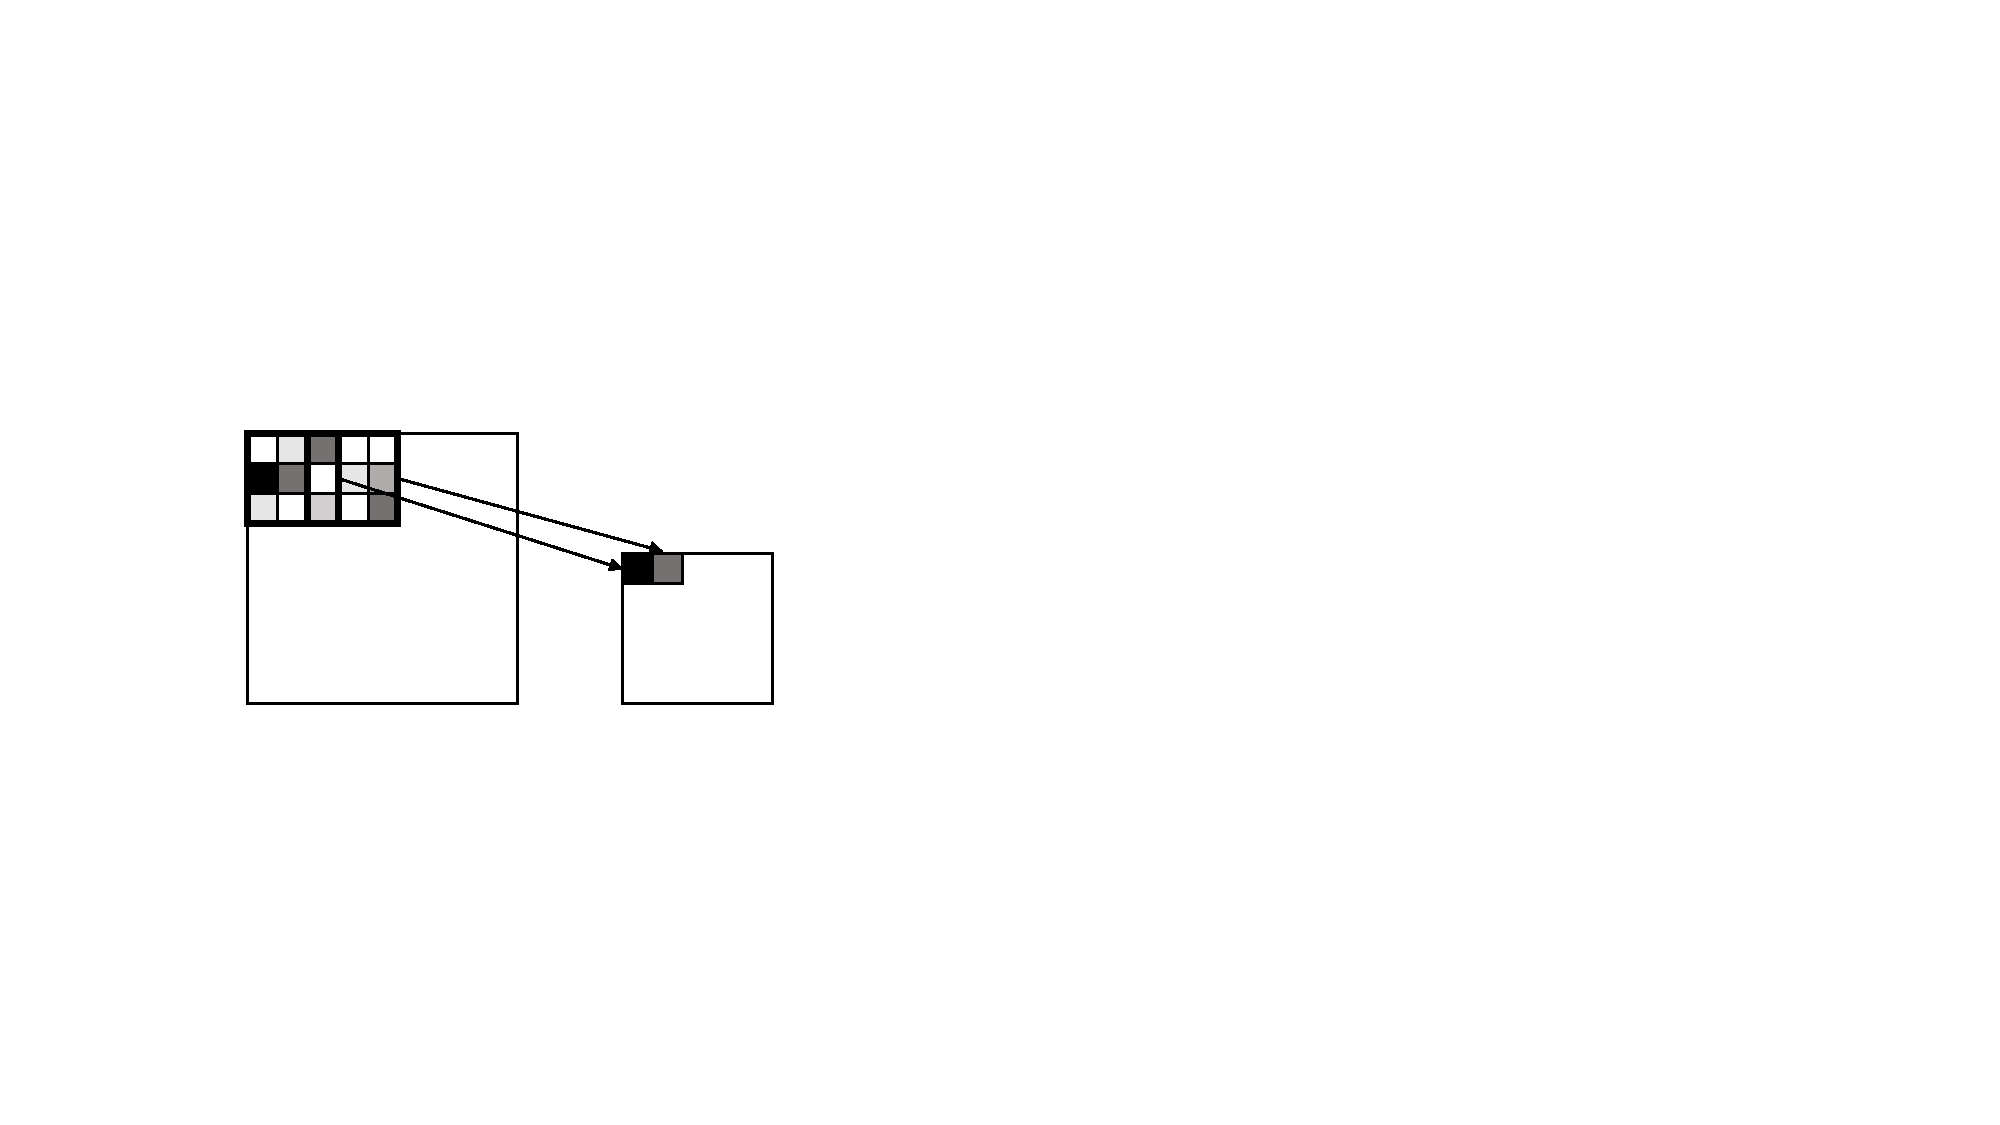
\includegraphics[width=0.4\linewidth]{./figures/pooling}
  \caption{$3 \times 3$ max pooling with a stride of two. }
  \label{fig_pooling}
\end{figure}

Since the convolution operation contains a large amount of computation, there are many techniques introduced to reduce it. A representative technique is applying the 2D convolution to the input image with a stride as shown in Figure~\ref{fig_stride}. A strided convolution performs down-sampling by sampling only every $s$ pixel in each direction of the input image, where $s$ is the value of the stride. Thus, the resulting feature-map size is smaller than the input image size. 

Another technique is \textit{pooling}. Pooling also performs down-sampling and reduces the amount of computation. It identifies a representative pixel for a pixel region to reduce the size of the input. For example, Figure~\ref{fig_pooling} shows $3 \times 3$ \textit{max pooling} with a stride of two. It divides the input in $3 \times 3$-pixel regions with a stride of two. For each region, it selects a pixel that has the maximum value in the region as the representative. 

\subsection{Convolutional Neural Networks}
\label{sec:CNN}
A \textit{convolutional neural network} (CNN) is an artificial neural network using convolutional filters to extract features from its input. In a CNN, a layer that performs 2D convolutions is called a \textit{convolutional layer}. Since a filter extracts a feature from the input image, a typical convolution layer extract multiple features from an input image using $N (\geq 1)$ filters, resulting in $N$ feature maps. Each of the feature maps is also called a \textit{channel}. The training stage of the CNN makes it learn a filter for each of the features.

\begin{figure}[htbp]
  \centering
  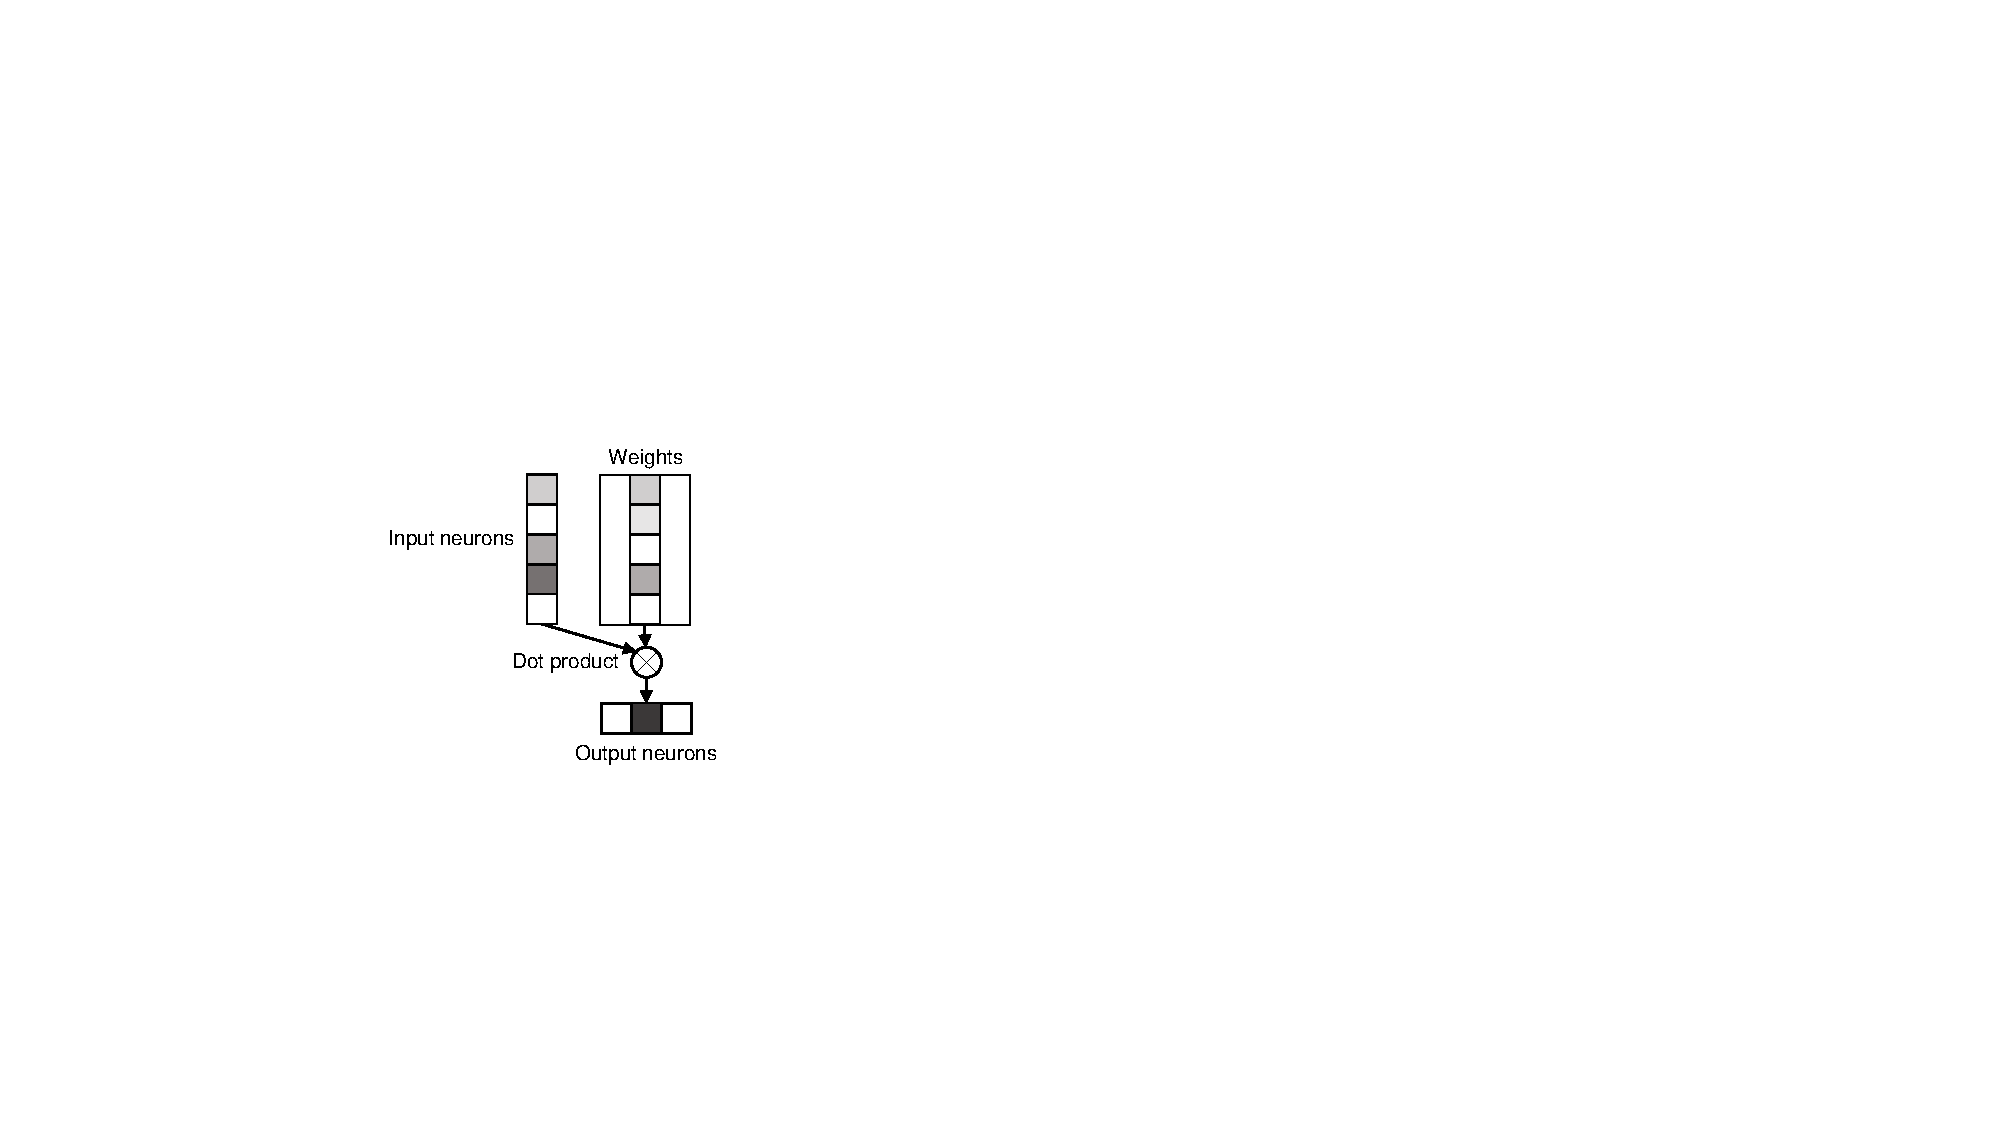
\includegraphics[width=0.5\linewidth]{./figures/fully}
  \caption{Computation in the fully connected layer. }
  \label{fig_fully}
\end{figure}

A \textit{fully connected layer} in a CNN combines the results of convolutions. As shown in Figure~\ref{fig_fully}, it consists of input neurons, output neurons, and weights that represent the relationship between the input and output. It performs matrix (the weights) and vector (the input) multiplication and generates the output.

\begin{figure*}[htbp]
  \centering
  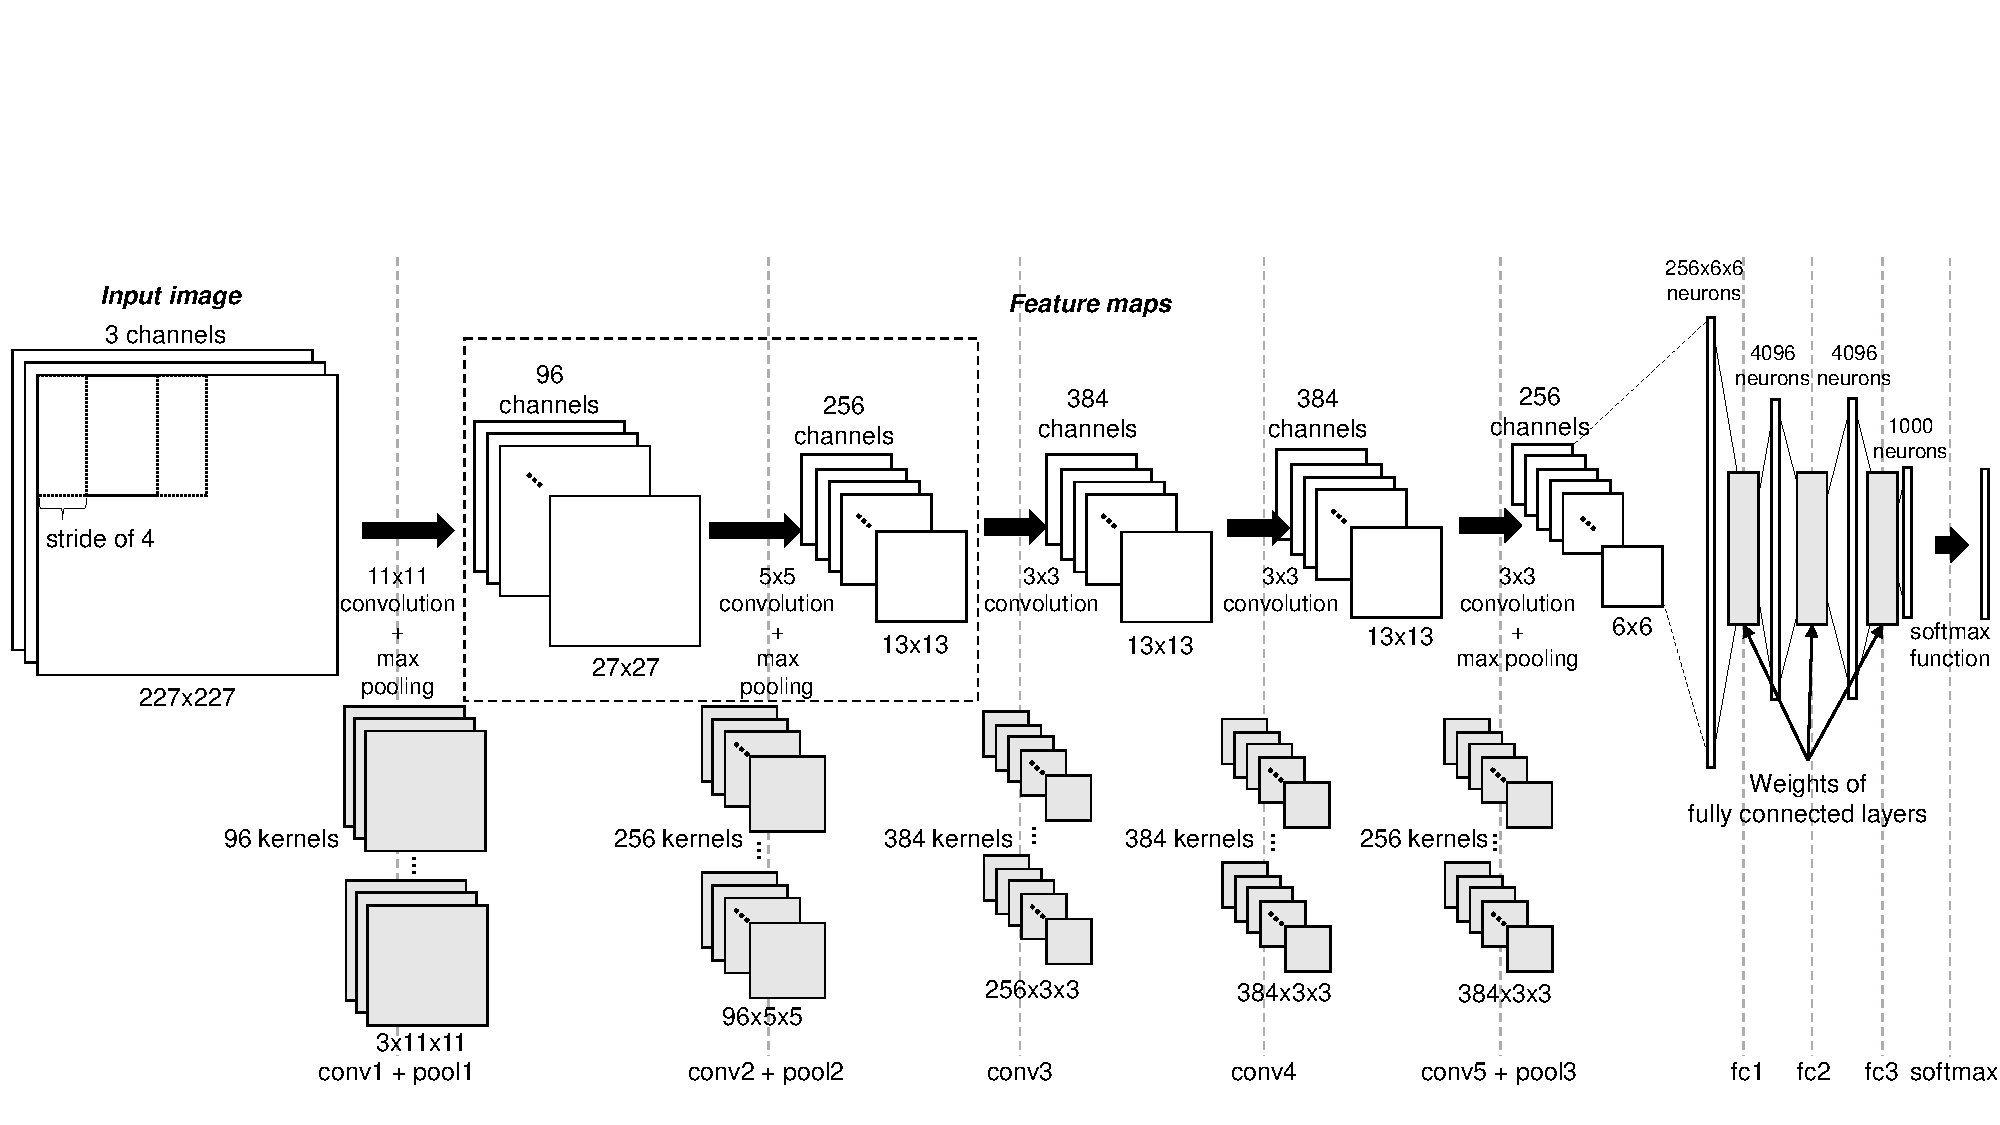
\includegraphics[width=\linewidth]{./figures/Alex}
  \caption{Organization of AlexNet.}
  \label{fig_Alex}
\end{figure*}

\begin{table}[htbp]
\centering
\caption{Configuration of AlexNet}
\label{alex_model}
\begin{scriptsize}
\begin{tabular}{l|l|l|l|l}
\hline
\begin{tabular}[c]{@{}l@{}}Layer\\name\end{tabular}    & 
 \begin{tabular}[c]{@{}l@{}}Kernel size\\ (pooling size) \\ / stride\end{tabular} 
 & Output size     & 
 \begin{tabular}[c]{@{}l@{}}Number of\\ parameters\end{tabular} & 
 \begin{tabular}[c]{@{}l@{}}Number of\\ FP \\operations\end{tabular} \\
\hline
conv1         & 11 x 11 / 4   & 96 x 55 x 55    & 35K        & 55G  \\
pool1         & 3 x 3 / 2     & 96 x 27 x 27    &           &      \\
conv2         & 5 x 5 / 1    & 256 x 27 x 27    & 614K   & 227G \\
pool2         & 3 x 3 / 2    & 256 x 13 x 13    &        &      \\
conv3         & 3 x 3 / 1    & 384 x 13 x 13    & 885K   & 65G  \\
conv4         & 3 x 3 / 1    & 384 x 13 x 13    & 1.3M   & 98G  \\
conv5         & 3 x 3 / 1    & 256 x 13 x 13    & 885K   & 65G  \\
pool3         & 3 x 3 / 2    & 256 x 6 x 6      &        &      \\
fc6           &              & 4096             & 37M    & 74M  \\
fc7           &              & 4096             & 16M    & 32M  \\
fc8           &              & 1000             & 4M     & 8M   \\
softmax       &              & 1000             &        &      \\ 
\hline 
\end{tabular}
\end{scriptsize}
\end{table}

{\bf AlexNet}. Figure~\ref{fig_Alex} shows a representative CNN, AlexNet\cite{krizhevsky2012imagenet}. It is one of the earliest successful CNNs that perform image recognition tasks using the ImageNet data set\cite{DBLP:journals/corr/RussakovskyDSKSMHKKBBF14}. It uses five convolution layers (\textsf{conv1}, \textsf{conv2}, \textsf{conv3}, \textsf{conv4}, and \textsf{conv5}) and three max pooling layers (\textsf{pool1}, \textsf{pool2}, and \textsf{pool3}) to extract features. In addition, there are three fully connected layers (\textsf{fc1}, \textsf{fc2}, and \textsf{fc3}) for image classification. Each layer uses the rectified linear unit (ReLU) for nonlinear neuron activation. 

Grey boxes in Figure~\ref{fig_Alex} represent kernels and weights of fully connected layers (\textit{i.e.}, network parameters) and white boxes represent the data produced by the layers. The input to \textsf{conv1} is the input image. The result of a previous convolution layer becomes the input to the next convolution layer after going through a max-pooling layer if there is any. At the beginning, 96 $3 \times 11 \times 11$ 3D kernels are applied to the RGB channels of the input image. This is equivalent to applying 96 $11 \times 11$ 2D kernels to each input image channel. 

The fully connected layers combine the features extracted by the previous convolution layers and creating a conclusion. The output of \textsf{fc3} after \textsf{pool3} becomes the input neurons of \textsf{fc1}. For a given image, AlexNet determines which image class the input belongs to among 1000 predefined image classes. The last layer, \textsf{softmax} layer, in AlexNet normalizes the output values of \textsf{fc3} and converts them to probability values. The \textsf{fc3} and \textsf{softmax} layers have 1000 output neurons, respectively, each of which corresponds to one of the image classes. The probability value of each \textsf{softmax} neuron represents the confidence level that the input image belongs to the associated class with the neuron.

\begin{figure}[htbp]
  \centering
  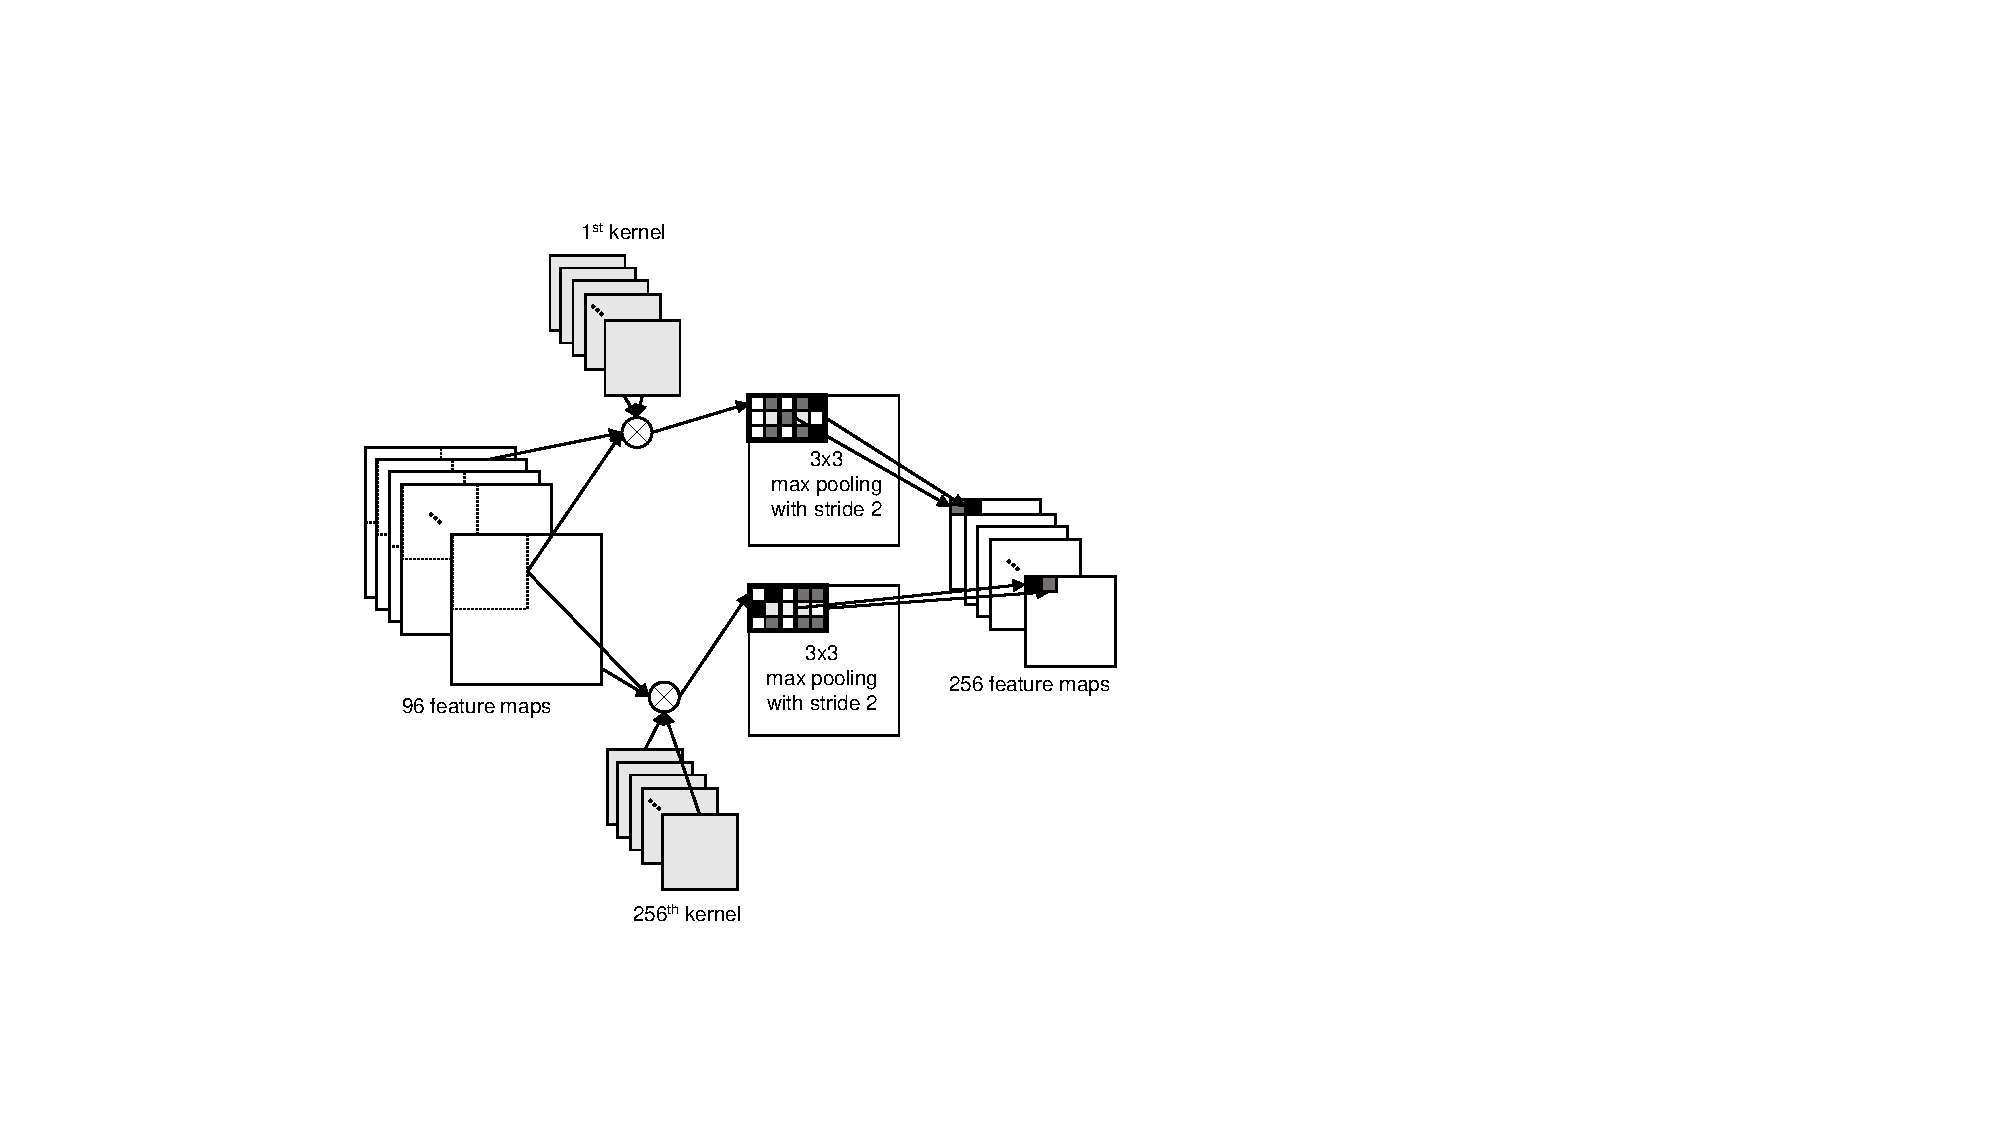
\includegraphics[width=\linewidth]{./figures/convolution}
  \caption{Convolution and max-pooling in the dotted box in Figure~\ref{fig_Alex}.}
  \label{fig_convolution}
\end{figure}

The dotted box in Figure~\ref{fig_Alex} (\textsf{conv2}+\textsf{pool2}) is detailed in Figure~\ref{fig_convolution}. The 96 feature maps produced by \textsf{conv1}+\textsf{pool1} are convolved by 256 $5 \times 5 \times 96$ 3D kernels and go through $3 \times 3$ max pooling with a stride of two resulting in 256 new feature maps. Since there are 96 inputs, applying a $5 \times 5$ 2D kernel to each of the 96 inputs is equivalent to applying a $5 \times 5 \times 96$ 3D kernel to the 96 inputs. The detailed configuration of the AlexNet model in this paper is presented in Table~\ref{alex_model}.

AlexNet has been frequently used for benchmarking deep learning libraries because it is equipped with most of the state-of-the-art DNN components, such as convolution, max-pooling, and dropout\cite{convnet-benchmarks}. The original AlexNet model includes a local response normalization (LRN) layer, but we exclude it in this paper because LRN is very rarely used in current CNNs. 

{\bf Training a CNN.} Training a CNN is a supervised learning process using training input images and correct class labels that are associated with the images. Since training a CNN is the most time consuming process, it is very important to reduce the training time of a CNN by efficiently implementing the CNN. The training phase has two stages: \textit{forward computation} and \textit{backward computation}. For a given training input image, the forward computation stage goes through the CNN layers from the first to the last and obtains the output from the last layer. For example, AlexNet determines the class to which the training input image belongs. After computing the difference between the output and the correct label, the backward computation stage obtains the values that need to be added to the network parameters (\textit{e.g.}, weights) of the last fully connected layer by computing gradients. After updating the parameters in the last layer with the gradients, these values are backward propagated to the previous layers (\textit{i.e.}, \textit{backpropagation} is performed) to adjust their parameters in the backward computation stage. The gradients are computed in the direction of minimizing the difference between the output of a layer and the correct answer for each layer.

{\bf Batch processing}. When a CNN is trained, training input images are divided into sets of images, each of which is called a \textit{batch}. A batch is processed by the CNN at a time. This is because the stochastic gradient decent technique (SGD)\cite{onlinesgd} that is typically used to obtain the gradients can be easily parallelized across different images in the same batch. 

{\bf 4D tensor format}. Since multiple 2D feature maps (or images) are typically processed in a layer at a time at a time, the feature map data in a CNN can be treated as four-dimensional tensors $<N, C, H, W>$, where $N$, $C$, $H$, and $W$ are the number of images in a batch, the number of channels (\textit{i.e.}, feature maps), the height of a feature map (or an image), and the width of a feature map (or an image), respectively. Since the 4D tensor data are stored in the order of the dimensions $N$, $C$, $H$, and $W$, they are called $NCHW$ 4D tensors. The computational complexity of convolving a $NCHW$ tensor with $K \times R \times S$ 3D kernel is $O(K \times CRS \times NHW)$.

\begin{figure}[htbp]
  \centering
  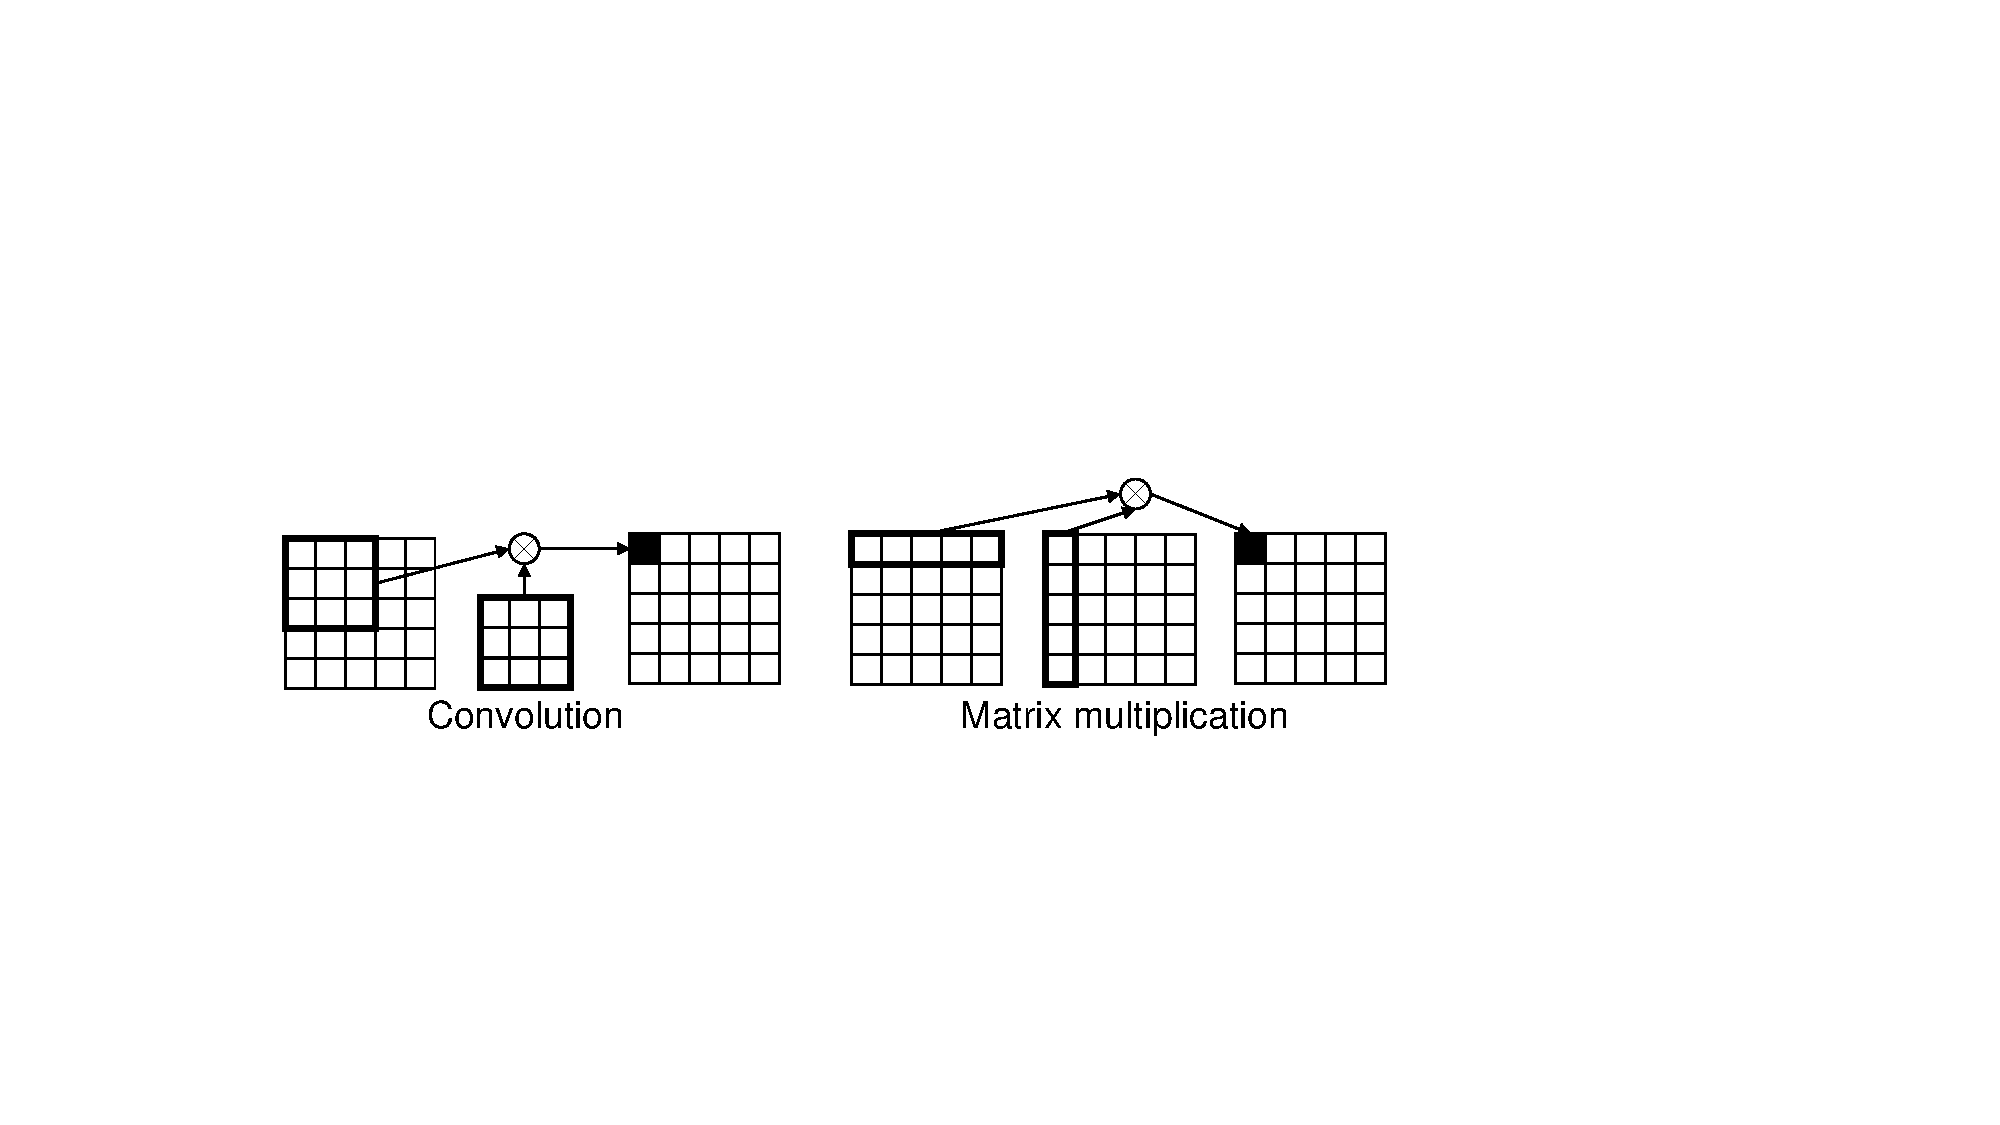
\includegraphics[width=0.9\linewidth]{./figures/direct}
  \caption{Direct convolution vs. matrix multiplication.}
  \label{fig_direct}
\end{figure}

\subsection{Convolution Algorithms}
\label{sec:algorithms}
{\bf Direct convolution}. Since the efficiency of computing a convolution is important to CNNs, several methods have been developed to efficiently implement the convolution operation. Directly computing the convolution (we call it \textit{direct convolution} in this paper) using Equation~\ref{2d-conv} is the most straightforward way to perform convolution. Cuda-convnet\cite{cuda-convnet} is a widely used direct convolution library. Figure~\ref{fig_direct} compares matrix multiplication and direct convolution computation.

\begin{figure}[htbp]
  \centering
  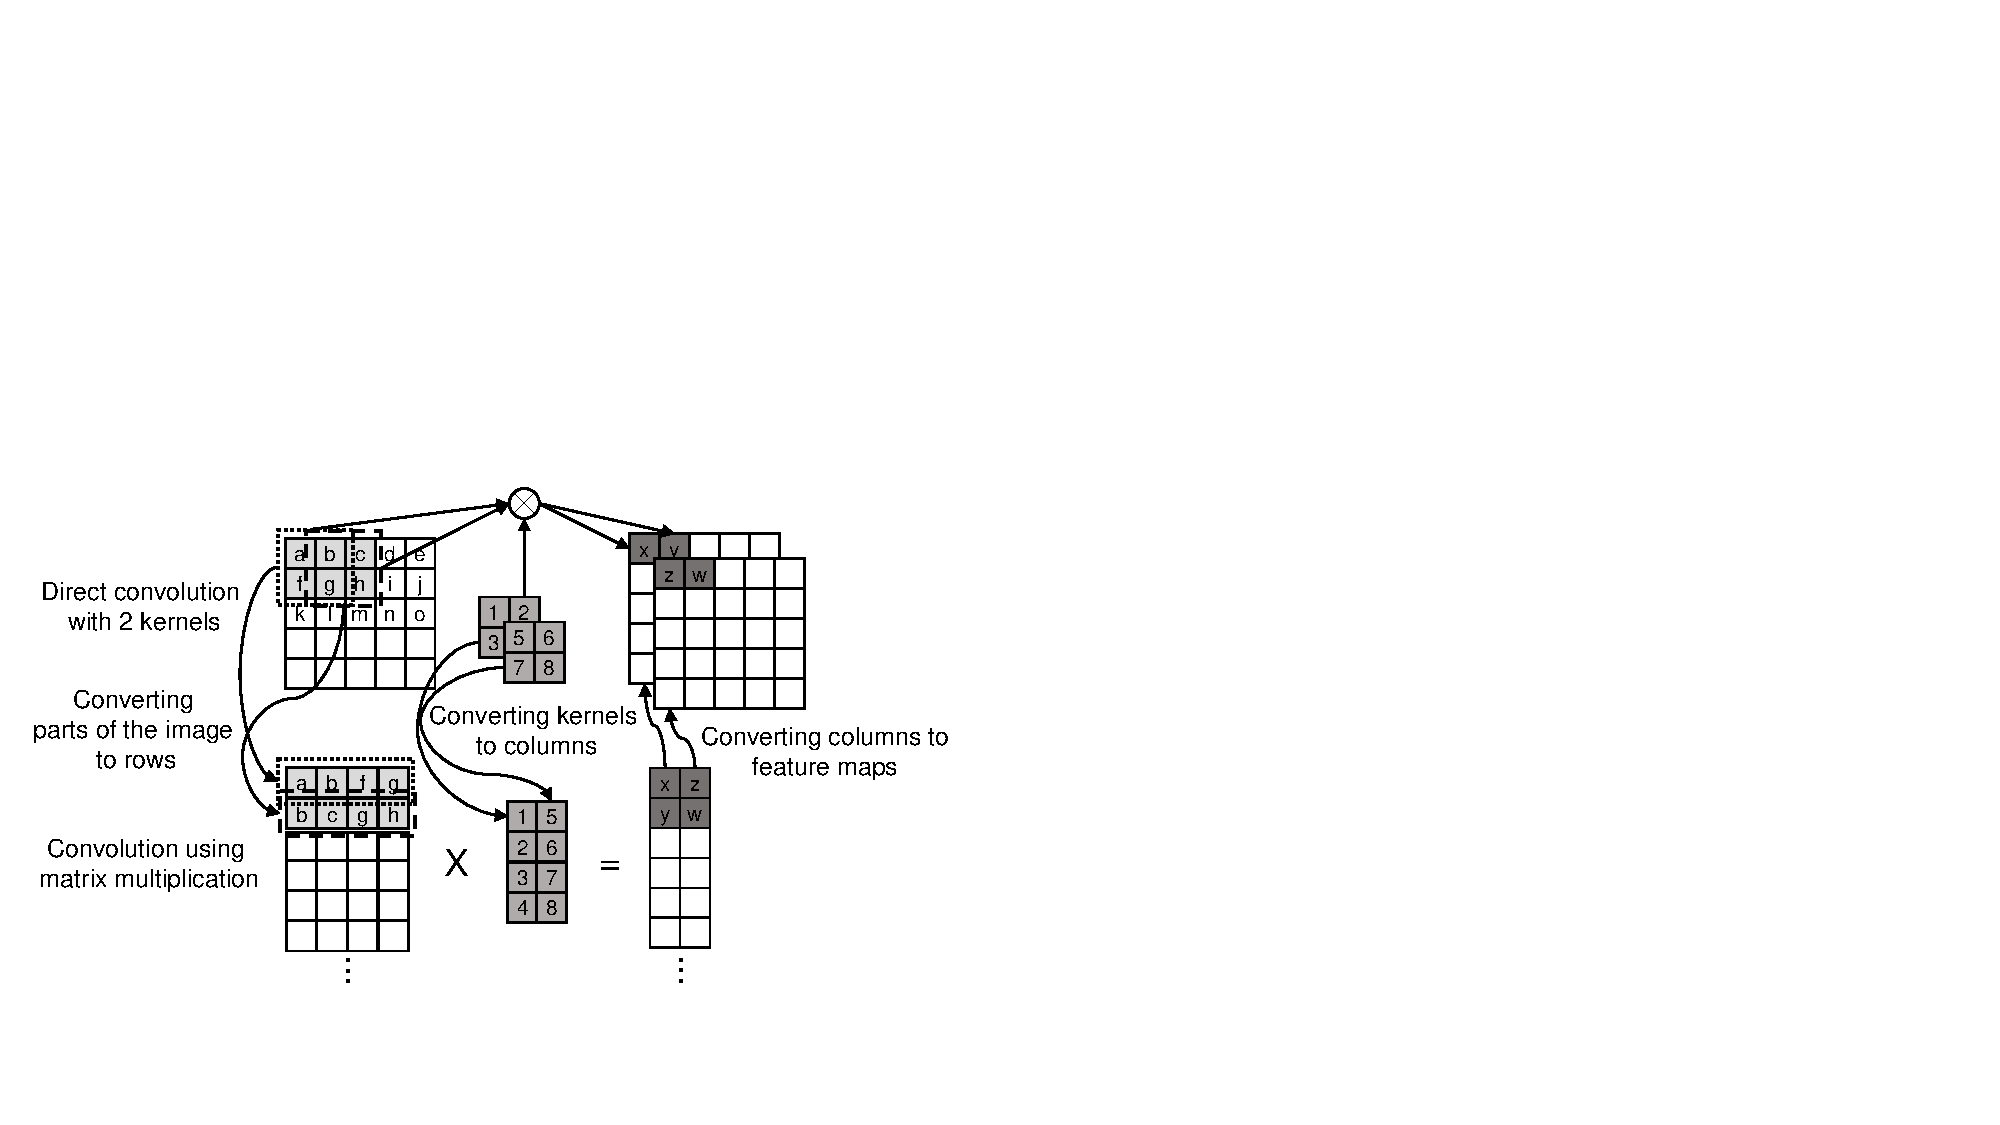
\includegraphics[width=\linewidth]{./figures/matmul}
  \caption{Convolution using matrix multiplication.}
  \label{fig_matmul}
\end{figure}

{\bf Using matrix multiplication}. CuDNN\cite{cudnn}, a DNN library from NVIDIA, treats the convolution as matrix multiplication (\textit{e.g.}, GEMM\cite{cublas}). Figure~\ref{fig_matmul} illustrates the process. It convolves a $5 \times 5$ image with two $2 \times 2$ kernels and obtains two $5 \times 5$ feature maps. When the input image has multiple channels, a row in the input matrix contiguously contains pixels from the multiple channels. When the number of input channels, the size of a kernel, the number of kernels, and the input image size are $C$, $R \times S$, $K$, and $H \times W$, respectively, the sizes of the input matrix and the kernel matrices become $CRS \times WH$ and $K \times CRS$, respectively. Since the complexity of the matrix multiplication is $O(K \times CRS \times WH)$, when the number of images in a batch is $N$, the complexity becomes $O(K \times CRS \times NWH)$. 

Interestingly, the computational complexity of this matrix multiplication method is the same as that of the direct convolution. However, matrix multiplication can be easily parallelized using highly efficient BLAS libraries\cite{cublas}. Moreover, it enables exploiting the GPU local memory that has  low latency and high bandwidth. cuDNN performs matrix multiplication by applying tiling to the matrices in the GPU local memory. This method scales well with a small batch size and can be used on all types of convolution layers. 

{\bf Using FFT}. The convolution operation can be implemented using a fast Fourier transform (FFT) algorithm to reduce computational complexity\cite{fftconv}. The complexity of FFT convolution is $O(K \times CWW \times \log W)$ that does not depend on the kernel size, $R \times S$. However, it requires more memory space because filters need to be padded to the dimension of the input. Another restriction is that it can be applied only to convolutions with the stride of one.

{\bf Using the Winograd algorithm}. Winograd convolution is based on GEMM\cite{cublas}. It reduces the complexity using Winograd's minimal filtering algorithm\cite{winograd}. It is similar to the well known Strassen's algorithm\cite{winograd1980arithmetic} for matrix multiplication. It reduces multiplication operations significantly when the kernel size is fixed. Thus, a different kernel size requires a different minimal filtering algorithm. The minimal filtering algorithm for $4 \times 3$ tiled matrix can reduce 12 multiplications to 6. Nesting the minimal filtering algorithm twice would reduce the algorithm complexity by a factor of 4\cite{winograd}. cuDNN 5.1 supports Winograd convolution only for the filter sizes of $3 \times 3$ and $5 \times 5$.

\subsection{Multi-GPU Support}
\label{sec:multiGPU-parallelism}
Multi-GPU support for DNNs can be implemented by exploiting \textit{data parallelism} or \textit{model parallelism}\cite{NIPS2012_4687}. Exploiting data parallelism means that input images in a batch are divided and distributed across multiple GPUs and processed by all the GPUs. Thus, all the GPUs have the entire network parameters. In the backward computation stage, each GPU computes its own gradients for the inputs assigned to it, then a single device (a CPU or a GPU) combines the gradients computed by all the GPUs and performs the SGD. Network parameters are updated with the result of the SGD, and they are distributed across the GPUs again. 

The communication cost in data parallelism depends on the number of network parameters. Since AlexNet has 62M parameters and their size is 250MB, each iteration (an iteration processes a batch) needs to transfer approximately 250MB of data per GPU. Quantization methods that approximate the value of a floating-point number with an integer can reduce the size of the data transfer\cite{deepcompress}. CNTK provides 1-bit SGD method that quantizes 32-bit gradient values into a single bit with some accuracy loss\cite{1-bit-stochastic-gradient-descent-and-application-to-data-parallel-distributed-training-of-speech-dnns}.

On the other hand, the model parallelism makes users to divide and distribute the network itself across GPUs. Since parameter updates can be done on each GPU, only a small amount of data needs to be communicated between GPUs. A convolution layer using carefully designed model parallelism typically outperforms data parallelism\cite{DBLP:journals/corr/YadanATR13}.

TensorFlow and Torch support both data parallelism and model parallelism. While Caffe and CNTK supports only data parallelism, the multi-GPU support of Theano is still in an experimental stage. Thus, we compare only the efficiency of data parallelism between Caffe, TensorFlow, Torch and CNTK for multiple GPUs. 

\subsection{Related Work}
Since it has been only a few years since deep learning frameworks were introduced to public, not that many previous studies compare their performance. Recently, some comparative studies for the deep learning frameworks are performed by Bahrampour \textit{et al.}\cite{DBLP:journals/corr/BahrampourRSS15} and Shi \textit{et al.}\cite{DBLP:journals/corr/ShiWXC16}. However, they show only the entire execution times of various DNN models built by the deep learning frameworks. They do not identify performance bottlenecks and reasons for performance differences. Moreover, they use cuDNN version R4 that does not support the Winograd convolution algorithm, and their work does not cover CNTK that was most recently introduced to public.

A benchmark result for some CNN frameworks is publicly available on GitHub\cite{convnet-benchmarks}. It reports forward and backward computation times of a CNN model. The latest result was produced with cuDNN version R4, while the most recent cuDNN version is R5.1. This paper uses cuDNN version R5 and R5.1.
